\documentclass[paper=a4, fontsize=11pt]{report} % A4 paper and 11pt font size
\usepackage[utf8]{inputenc}
\usepackage[T1]{fontenc} % Use 8-bit encoding that has 256 glyphs
\usepackage[english]{babel} % English language/hyphenation
\usepackage{amsmath,amsfonts,amsthm} % Math packages

\usepackage{graphicx}
\usepackage{siunitx}

\usepackage[nottoc]{tocbibind}

\usepackage[backend=bibtex]{biblatex}
\bibliography{bibtexlibs}

\usepackage{sectsty} % Allows customizing section commands
\allsectionsfont{\centering \normalfont\scshape} % Make all sections centered, the default font and small caps

\usepackage{fancyhdr} % Custom headers and footers
\pagestyle{fancyplain} % Makes all pages in the document conform to the custom headers and footers
\fancyhead[L]{GROUP TITLE} % No page header - if you want one, create it in the same way as the footers below
\fancyfoot[L]{} % Empty left footer
\fancyfoot[C]{} % Empty center footer
\fancyfoot[R]{\thepage} % Page numbering for right footer
\renewcommand{\headrulewidth}{0pt} % Remove header underlines
\renewcommand{\footrulewidth}{0pt} % Remove footer underlines
\setlength{\headheight}{13.6pt} % Customize the height of the header

\usepackage{hyperref}
\hypersetup{
    colorlinks,
    citecolor=black,
    filecolor=black,
    linkcolor=black,
    urlcolor=black
}

\fancypagestyle{firststyle}
{
  \fancyhf{}
  \fancyfoot[R]{\thepage}
}

\newcounter{alphasect}
\def\alphainsection{0}

\let\oldsection=\section
\def\section{%
  \ifnum\alphainsection=1%
    \addtocounter{alphasect}{1}
  \fi%
\oldsection}%

\renewcommand\thesection{%
  \ifnum\alphainsection=1% 
    \Alph{alphasect}%
  \else
    \arabic{section}%
  \fi%
}%

\newenvironment{alphasection}{%
  \ifnum\alphainsection=1%
    \errhelp={Let other blocks end at the beginning of the next block.}
    \errmessage{Nested Alpha section not allowed}
  \fi%
  \setcounter{alphasect}{0}
  \def\alphainsection{1}
}{%
  \setcounter{alphasect}{0}
  \def\alphainsection{0}
}%


\numberwithin{equation}{section} % Number equations within sections (i.e. 1.1, 1.2, 2.1, 2.2 instead of 1, 2, 3, 4)
\numberwithin{figure}{section} % Number figures within sections (i.e. 1.1, 1.2, 2.1, 2.2 instead of 1, 2, 3, 4)
\numberwithin{table}{section} % Number tables within sections (i.e. 1.1, 1.2, 2.1, 2.2 instead of 1, 2, 3, 4)

%------ Listings --------------
\usepackage{color}
\definecolor{light-gray}{gray}{0.95}
\definecolor{orange}{rgb}{1, 0.5, 0}
\usepackage{listings}

\lstnewenvironment{code}[1][]%
{\minipage{\linewidth}
\lstset{ %
language=C,  % choose the language of the code
basicstyle=\footnotesize,       % the size of the fonts that are used for the code
numbers=left,                   % where to put the line-numbers
numberstyle=\footnotesize,      % the size of the fonts that are used for the line-numbers
stepnumber=1,                   % the step between two line-numbers. If it is 1 each line will be numbered
resetmargins=true,              % reset line numbers
numbersep=5pt,                  % how far the line-numbers are from the code
backgroundcolor=\color{white},  % choose the background color. You must add \usepackage{color}
showspaces=false,               % show spaces adding particular underscores
showstringspaces=false,         % underline spaces within strings
showtabs=false,                 % show tabs within strings adding particular underscores
frame=single,                   % adds a frame around the code
tabsize=2,                      % sets default tabsize to 2 spaces
captionpos=b,                   % sets the caption-position to bottom
breaklines=true,                % sets automatic line breaking
breakatwhitespace=false,        % sets if automatic breaks should only happen at whitespace
escapeinside={\%*}{*)},         % if you want to add a comment within your code
identifierstyle=\color{blue},
stringstyle=\color{orange},
#1
}}%
{\endminipage}


%----------------------------------------------------------------------------------------
%   TITLE SECTION
%----------------------------------------------------------------------------------------

\newcommand{\horrule}[1]{\rule{\linewidth}{#1}} % Create horizontal rule command with 1 argument of height

\title{ 
\normalfont \normalsize 
\textsc{Norwegian University of Science and Technology} \\ [25pt] % Your university, school and/or department name(s)
\horrule{0.5pt} \\[0.4cm] % Thin top horizontal rule
\huge \textbf{Demolicious} \\ % The assignment title
TDT4295 Computer Design Project\\
\horrule{2pt} \\[0.5cm] % Thick bottom horizontal rule
}

\author{Authors:\\ \\
Aleksander Gustaw Wasaznik\\
Aleksander Vognild Burkow\\
Kristian Fladstad Normann\\
Christoffer Tønnessen\\
Andreas Løve Selvik\\
Julian Ho-yin Lam\\
Eirik Jakobsen\\
Stian Jensen\\
Torkel Berli}

\date{\normalsize November 19, 2014}

\begin{document}

\pagenumbering{roman}

\maketitle

\newpage

%blank page
\vspace*{\fill}
\begin{center}
    [This page is intentionally left (almost) blank.]
\end{center}
\vspace*{\fill}


\thispagestyle{firststyle}

\newpage

%ABSTRACT
\documentclass[../main/report.tex]{subfiles}
\begin{document}
\chapter*{Abstract}
\label{sec:abstract}

\vspace*{\fill}

Demolicious is a general purpose SIMT inspired computer.
It is specialized to handle parallel rendering of computer graphics.
The performance of the system scales linearly with the amount of cores.

In addition this system is the first of its kind in this project with an HDMI output.
Computer generated graphics was chosen as a showcase application, and was successfully shown on a HDMI enabled screen.

Also this is the first computer to make use of cross clock domain design.

A backup oriented design philosophy for the PCB was chosen as the philoshoply with highest likelyhood of success.
It has been implemented on a PCB, and passed testing and verification.

\vspace*{\fill}
\end{document}


\newpage

\tableofcontents

\setcounter{secnumdepth}{3}

\newpage

\pagenumbering{arabic}

\part{Introduction}

%INTRODUCTION
\section{Introduction}

Introduction citation \cite{example}.


% STATE OF THE ART
\documentclass[../main/report.tex]{subfiles}
\begin{document}
\chapter{State of the Art}

Yo.
\end{document}

\part{Solution}

% System Overview
\chapter{System Overview}

\section{Physical system structure}

\section{Logical system structure}

\section{Programming model}


% CPU
\documentclass[../main/report.tex]{subfiles}
\begin{document}
\chapter{CPU}

The main control unit of the Demolicious computer is the CPU, implemented on an EFM32GG Microcontroller. Host programs, as described in the previous chapter, will run on the CPU,
and can upload and launch kernels on the GPU.
The CPU provides a framework of utility functions for interfacing the GPU.

\subfile{../cpu/functionality.tex}

\subfile{../cpu/bus.tex}

\subfile{../cpu/load-kernel.tex}

\subfile{../cpu/run-kernel.tex}

\subfile{../cpu/load-constant.tex}

\end{document}


% GPU
\documentclass[../main/report.tex]{subfiles}
\begin{document}

\chapter{GPU}

The GPU is at the heart of the Demolicious system.
Inspired by SIMD and SIMT architecture and programming models, the GPU architecture is named 'GhettoCUDA' in honor of NVIDIAs CUDA environment.\todo{cite this}

The GhettoCUDA architecture is highly parallel, in that it allows for a great number of threads to execute in parallel on multiple streaming processors.
A thread is the unit of execution, in essence a single procedure, that when correctly parameterized by run-time values allows for the transformation of a set of input data to a graphical representation to be visualized by the HDMI module.
A simple kernel, requiring no input, might be one that for each pixel in the framebuffer stores the color red.

The main design challenge in creating a GPU-inspired system is managing to saturate the memory bus as much as possible, changing memory access patterns from clustering together in time to a more spread-out pattern.
To facilitate this, the architecture allowing for multiple threads to execute on each streaming processor core, with a staggered start.
This design decision allows for a steady stream of load/store instructions without requiring a system stall as one waits for memory requests to return.

\section{Responsibilities}

The GPU has these responsibilities
\begin{enumerate}
  \item
    Receive instructions and constants from the CPU
  \item
    Handle kernel invocations from the CPU
  \item
    Write results to external SRAM
  \item
    Assert the 'computation finished' signal to the CPU
\end{enumerate}

\section{Architecture Overview}
\begin{figure}[H]
\centering
\includegraphics[width=\textwidth]{../gpu/diagrams/architecture_overview.png}
\caption{A high level overview of the GPU.}
\label{fig:architecture_overview}
\end{figure}
Figure \ref{fig:architecture_overview} presents a high level overview over the GPU.
The CPU issues commands to the communication unit in the GPU. Commands are launching a kernel, uploading kernels to the instruction memory, writing to the constant memory, and read/write to SRAM.
Instructions are fetched from the instruction memory and decoded by the control unit, which has the responsibility of setting the control signals for the instructions.
The processors load constants from the constant memory, and uses the load/store unit for accessing the data memory.


\section{Receiving a Kernel Call}
\begin{figure}[H]
\centering
\includegraphics[width=\textwidth]{../gpu/diagrams/receiving_a_kernel_call.png}
\caption{Launching a kernel from the GPU's viewpoint.}
\label{fig:kernel_call}
\end{figure}

The communication unit is responsible for receiving kernel call requests from the CPU.
When a kernel call is received, the kernel launch signal is asserted.
A kernel call consists of the address of the kernel, and the number of threads to launch.

The kernel launch signals are forwarded to the thread spawner, which writes the kernel start address to the PC register, and starts distributing thread IDs to the processor cores. 
After holding the kernel launch signals high, the communication unit has completed its role in launching the kernel.
When the kernel completes executing, the thread spawner asserts the kernel done signal, and the communication unit forwards the signal to the CPU, indicating that the kernel call has completed.


\section{Running a Kernel}
Once the thread spawner has been initiated by the communication unit, the kernel runs to completion without intervention by the CPU. 
When a kernel run starts, the thread spawner assigns thread IDs to each warp in the barrel.
After the initial IDs have been assigned the GPU enters normal execution.
\begin{figure}[H]
	\centering
	\includegraphics[width=0.9\textwidth]{../gpu/diagrams/kernel_run_state_machine.png}
	\caption{The GPU's internal state during kernel execution.}
	\label{fig:kernel_run_state_machine}
\end{figure}
A normal kernel execution can be represented by the state machine in figure \ref{fig:kernel_run_state_machine}.
During the kernel execution stage the threads in a warp execute the same instructions, until the control unit encounters a \emph{finished} instruction.
Upon receiving a \emph{finished} instruction the control unit asserts the \emph{finished} signal alerting the thread spawner that a new warp has to be spawned.
The thread spawner keeps track of the number of threads awaiting launch.
When the thread spawner receives a \emph{finished} instruction and no more warps are awaiting launch, the kernel complete signal is asserted, and the kernel run has completed.


\section{Module Details}

\subfile{../gpu/core.tex}

\subfile{../gpu/thread-spawner.tex}

\subfile{../gpu/regdir.tex}

\subfile{../gpu/sram.tex}

\subfile{../gpu/lsu.tex}

\subfile{../gpu/hdmi.tex}

\end{document}


% Comm
\documentclass[../main/report.tex]{subfiles}
\begin{document}

\chapter{On-Chip Communication Modules}

\section{Communication Unit}

\section{HDMI Unit}
\subfile{../comm/hdmi.tex}

\section{SRAM Arbiter}

\end{document}

%PCB
\documentclass[../main/report.tex]{subfiles}
\begin{document}

\chapter{Physical Implementation}
\label{sec:pcb}

This chapter will describe the PCB layout, the main components and the design philosophy that went into solving the system requirements.
%\section{Layout Overview}
\documentclass[../main/report.tex]{subfiles}
\begin{document}

\section{Physical system structure}

\missingfigure{Physical overview}

\end{document}

\section{Design for Redundancy}

When designing a system the PCB is one of the harder things to debug.
If a wire inside the PCB is wrong, there is not munch that can be done, except buying a new PCB.
This becomes apparant when seeing most projects only have a working PCB on the 3rd of maybe even the 4th try.
Because of this, a strong philosophy has been used in the design for the PCB, as shown in figure \ref{fig:pcb_philosophy}.

To make sure the propability that a pcb will have a working design will be as high as possible, all aspects of the PCB has one or more backup plans.
All important wires and unused pins have been put onto headers, which can be rerouted manually.
That way each part can be connected to other parts of the board, or to other sources.
Because of this, the board is not optimized for size, but was rather made to optimize for highest possible chance of success.

Another part of this design is that each vital part of the PCB follows a modular design.
Each isolated part will work on its own, with the help of other components, if the rest of the board fails.
A PCB with a broken MCU, but with a functioning FPGA can be connected together and work as one system none the wiser.

\section{Main Components}

\subsection{Microcontroller / System Control Unit}
The EFM32 Giant Gecko 32-bit Microcontroller from Energy Micro was chosen as the controller for this project.
A microcontroller from Energy Micro was required for the task and this particular controller is
very energy efficient, which is a plus.
In addition to this, there were a lot of development boards available,
plus over half of the group had experience with this controller from the subject
TDT4258 Energy Efficient Computer Systems.

The EFM32GG990F512-BGA112 was chosen as a powerful enough version of the microcontroller.

\subsection{FPGA}
The XC6SLX45-2CSG324I FPGA of the Spartan-6 family from Xilinx was chosen as the FPGA.
This particular FPGA has been used for different tasks on the university before, and the support systems are therefore available to us.
The version was the one used on the PCB.
A less powerful version of this one was available for testing on development boards in the lab.

\section{Input}

The main source of data communication between microcontroller and a host PC is USB.
This protocol has been used for years on projects like these, with good results. \todo{citation needed}

However, if the USB fails, there are backup plans.
Primarily a serial port (RS-232) has been included to work if the USB should fail.
If this also fails, the wires from the serial port is put on headers, which can be used as GPIO pins.

\section{Output}
The main source of output from the FPGA is an HDMI connector.
This is a novel feature this year, as no previous group has tried to implement it before.

Because of this new challenge, a lot of backup schemes were put in place.
The HDMI connector is put on headers, in case the connector fails.
A separate VGA module is connected to the FPGA, in case the HDMI doesn't work and if this fails, a VGA module is also connected to the microcontroller.

\section{Power}
USB connection with successive headers that allow for using an external power supply in case power fails.

\section{Bus}
Standard EBI connection between FPGA and MCU, but with headers in between such that external connection can be done in case of failure on one side of the connection, as well as an easy way to check transmitted signals during debugging.

\section{Clocks}
FPGA oscillator along with header on which an external oscillator resource can be connected by way of backup.
The microcontroller clocks on the other hand have a backup solution in that the microcontroller has internal RC-oscillators for use in case the crystals malfunction.


\section{Footprints}
Predominantly SMDs(surface mounted device) large enough for humans to solder(with a couple of exceptions)

\subfile{../pcb/hdmi.tex}

\todo{...Uncertain ie om at vi endra litt på en del footprints, men pga hvordan fysiske komponenter funker,}

\subsubsection{Prebundled}

\subsubsection{Handmade}
Some footprints we had to make ourselves.
This was done inside Altium.
The specification for the footprints was found in the datasheets of the component in question.

When making the handmade footprints some other thoughts were taken into account.

\begin{itemize}
    \item We need to solder these components
    \item The connection on the components is physical, as long as it leads current, it will work.
    \item Some datasheets didn't match the component exactly, but was for a sister component
\end{itemize}

With this in mind we made footprints which was slightly bigger than it needed to.

\begin{verbatim}
Needed:                 Actual:
--------------          --------------
|            |          |            |
|--|      |--|       |--|--|      |--|--|
|  |      |  |       |  |  |      |  |  |
|..|      |--|       |--|..|      |--|--|
|            |          |            |
--------------          --------------
\end{verbatim}
>>>>>>> Add intro footprint
\end{document}


\part{Results \& Discussion}

% TESTING
\documentclass[../main/report.tex]{subfiles}
\begin{document}

\chapter{Testing}

Does it work?

\section{VHDL system integration tests}

Before deploying to an actual FPGA, it is important to ensure correct behavior in system-level testbenches.
This testing is valuable, as if one can verify correct behavior in simulation, one has fewer potential errors when debugging the FPGA itself.

System tests for each of the major datapaths through the design have been created and run successfully.
The result of each test is verified by comparing all pixels in the framebuffer after the kernel has been run, to precomputed values in Isim.

\subsection{Memory stores and kernel parameterization}

To verify that stores to memory, as well as constant memory, actually works, the kernel presented in listing \ref{lst:param-color-kernel} is used as a system test.
It has been relisted in listing \ref{lst:test-param-kernel} for convenience.
If successful, this allows for parameterizing kernel behaviour with values loaded at runtime, reducing the need for recompilation.

\begin{assembly}[caption={Kernel to test constant memory and parameterization}, label=lst:test-param-kernel]
ldc $data, 0
mv $address_lo, $id_lo
mv $address_hi, $id_hi
sw
thread_finished
\end{assembly}

Expected behavior of test:
\begin{enumerate}
  \item
    The color green should successfully be loaded from constant memory.
  \item
    It should be stored to memory.
  \item
    The screen should be filled with the color green.
\end{enumerate}

\subsubsection*{simulation results}

\begin{figure}[H]
  \centering
  \begin{subfigure}[b]{\textwidth}
    \includegraphics[width=\textwidth]{../testing/assets/Constant_load_&_store.png}
    \caption{Isim simulation showing constant load and store word}
    \label{fig:isim-kernel-parameterization}
  \end{subfigure}
  \begin{subfigure}[b]{0.3\textwidth}
    \includegraphics[width=\textwidth]{../testing/assets/green_screen.jpg}
    \caption{LX16 run}
    \label{fig:LX16-kernel-parameterization}
  \end{subfigure}
  \caption{Results from simulation and LX16 of fillscreen kernel}
\end{figure}

In the left yellow square of figure \ref{fig:isim-kernel-parameterization}, one can see the load constant instruction being executed (0x08050000) in barrel line 1.
The Constant to reg signal is asserted, and the constant value 0x07E0 is passed into the register write data signal.

In the right yellow square, the store word instruction (0x100000000) executes in barrel line 0.
The LSU accepts the write request same cycle (LSU write request goes high), and two cycles later the request packet reaches the LSU data line.
The LSU asserts LSU write\_n, (the signal is active low), and external RAM handles the store request.

The testbench passes, and values have now been successfully written to memory.
It also runs on actual hardware, the result shown in figure \ref{fig:LX16-kernel-parameterization}.

\subsection{Masked instruction execution}

Masked instructions are used to allow for some degree of conditional execution in the lack of proper branching and jumps.
This requires that the architecture actually respects the mask bit when set.
The masked execution kernel presented earlier in listing \ref{lst:lst:masked-execution} is used for this test.
It has been relisted in listing \ref{lst:test-masked-execution} for convenience.

\begin{assembly}[caption=Conditional execution using predicated instructions, label=lst:test-masked-execution]
ldc $10, 0 ; Load color one
ldc $11, 1 ; Load color two
srl $mask, $id_lo, 6 ; Shift to the right converts ID to y pos
mv $data, $10
? mv $data, $11 ; Will only be executed every other row
mv $address_lo, $id_lo
mv $address_hi, $id_hi
sw
thread_finished
\end{assembly}

Expected behavior of test:
\begin{enumerate}
  \item
    Each row should be colored according to the last bit of their y position.
\end{enumerate}

\subsubsection*{simulation results}

\begin{figure}[H]
  \centering
  \begin{subfigure}[b]{\textwidth}
    \includegraphics[width=\textwidth]{../testing/assets/masking-yes.png}
    \caption{Isim simulation showing successful masking.}
    \label{fig:isim-masked-execution}
  \end{subfigure}
  \begin{subfigure}[b]{0.3\textwidth}
    \includegraphics[width=\textwidth]{../testing/assets/lines.jpg}
    \caption{LX16 run}
    \label{fig:LX16-masked-execution}
  \end{subfigure}
  \caption{Results from simulation and LX16 of masked execution}
\end{figure}

In the left yellow square of figure \ref{fig:isim-masked-execution}, we can see the \verb/srl/ instruction being executed (0x00023181). As this thread has thread id 192, the result out is 3.
The low bit is stored into the mask register, enabling masking for this thread.

In the middle yellow square, barrel 0 is once again active, and we can see that the predicate bit of core 0 has been asserted.
As this instruction isn't masked, the predicate bit is ignored and the value of 001f is stored into the data register.

In the right yellow square, the conditional data move is executed (0x81602804).
As the mask enable signal goes high, the register write enable signal is pulled low due to the predicate bit, resulting in the data not being written to registers.

The testbench passes, and predicated instructions are not executed when masking is enabled.
As can be seen in figure \ref{fig:LX16-masked-execution}, the kernel runs on actual hardware, and every second line is colored differently.

\subsection{Loads from primary memory}

\subsection{Kernel square}

\subfile{../testing/io_testing.tex}

\subfile{../testing/pcb-testing.tex}

%\subsection{JTAG test}
%In these tests we attempted to connect to respectively, the FPGA and the MCU by way of the appropriate headers, thereby verifying that they had been properly soldered in place and were functional.
%\subfile{../testing/JTAG_test.tex}

\end{document}


% RESULTS
\documentclass[../main/report.tex]{subfiles}
\begin{document}

\chapter{Results}

\begin{figure}[H]
	\centering
	\includegraphics[width=\textwidth]{../results/diagrams/frankenlicious.jpeg}
	\caption{The working Demolicious devkit setup}
	\label{fig:frankenlicious}
\end{figure}

In this section, the fruit of our labor, namely the Demolicious system is presented.
The system has been sucessfully run on a concoction of FPGA and MCU devkits, using the HDMI port of the PCB for video output.
This setup is showcased in figure \ref{fig:frankenlicious}.

A PCB version is almost fully operational.
A version with both FPGA and MCU flashed with their respective images managed to output animations, with some undiagnosed showstopping software glitches.
The venture had to be paused due to a lack of time towards the end of the project.

Kernel images presented in this section are taken from the same setup presented in figure \ref{fig:frankenlicious}.

\section{Scalability of the Demolicious system}
\label{sec:scalability}

The architecture of the Demolicious system easily scales to a larger number of processors.
As there is a linear relationship between the number of processor cores on chip and processor throughput, one can simply add more cores to increase performance.

Limiting factors to this scalability include:
\begin{enumerate}
  \item
    The more cores, the lower the clock frequency, as signal propagation time and fanout increases
  \item
    Space available on the chosen FPGA
  \item
    Power consumption constraints, as more cores increase active power consumption
\end{enumerate}

\begin{table}[H]
\begin{tabularx}{\textwidth}{cccccc}
\hline
Cores & Crit. path & Max freq. & Dynamic+quiescent power & LX16 & LX45 \\
\hline
\hline
2      & 17.103ns      & 58.469MHz & \SI{0.272}{W}: 0.088 + 0.184 & \checkmark & \checkmark  \\
4     & 17.959ns      & 55.682MHz & \SI{0.292}{W}: 0.107 + 0.184 & \checkmark & \checkmark \\
8   & 19.722ns      & 50.108MHz & \SI{0.353}{W}: 0.168 + 0.186 & X          & \checkmark \\
16     & X  & X & X        & X & X \\
       &               &           &                   &    & \\
\hline
\end{tabularx}
\caption{Hardware configurations compared. Harvested from post place \& route static simulation.}
\label{table:scalability}
\end{table}

The 4-core design fits with room to spare on the LX16, but does not fit the 8-core design.
The LX45 shifts this up one notch, fitting the 8-core design, but being unable to place \& route the 16-core design.
For all processor designs, the critical path passes from the immediate field of the instruction through the ALU into the active register file.
This is something that could be increased drastically by pipelining the processor.

Figure \ref{table:scalability} shows that there is a negligible drop in maximum frequency from two to eight cores.
At 50.108MHz with 8 cores, the GPU has an instruction throughput of ~400 mips.
This compares favorably to the ~117 mips of the two-core architecture.

It does however come with a 100mAh increase in power draw.
Luckily this only constitutes a 30\% total increase in power, considerably less than the fourfold improvement in GPU throughput.
The decrease in execution time will allow both the host CPU and the GPU to enter lower power states quicker, reducing static power consumption.

\section{Performance}

In the Demolicious system, the kernel calls can be issued by the CPU in only a few cycles.
This means that the number of frames per second (FPS) that the system can display is dominated by the run time of the kernels.

\begin{figure}[H]
	\centering
	\begin{subfigure}[t]{0.45\textwidth}
		\centering
		\includegraphics[width=\textwidth]{../results/diagrams/green_screen_run.jpg}
		\caption{Output from the green screen kernel.}
	\end{subfigure} 
	\begin{subfigure}[t]{0.45\textwidth}
		\centering
		\includegraphics[width=\textwidth]{../results/diagrams/kernel_run_tunnel.jpg}	
		\caption{Output from the tunnel kernel (Listing \ref{lst:tunnel-kernel}).}
	\end{subfigure}
	\caption{Running two example kernels.}
	\label{fig:kernel_outputs}

\end{figure}

Figure \ref{fig:kernel_outputs} shows the output from the green screen kernel, and the more complex tunnel effect kernel.
It's desirable that both these kernels can be run at about 30 FPS.
Using the results presented in section \ref{sec:scalability}, the expected frames per second for varying resolutions can be estimated.

\begin{figure}[H]
	\centering
		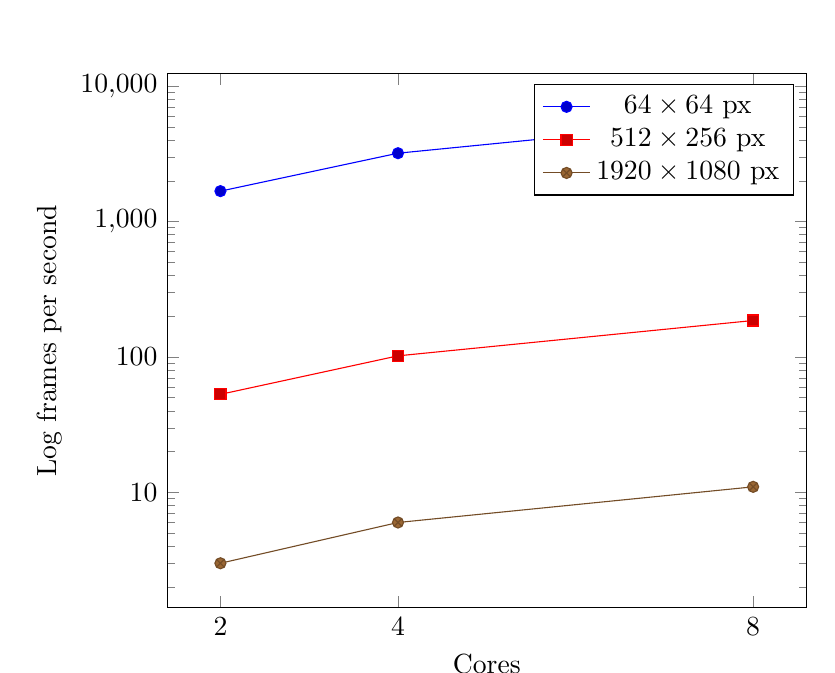
\begin{tikzpicture}
		   \begin{semilogyaxis}[
		   	   width=0.8\textwidth,
			   log ticks with fixed point,
		       xlabel=Cores,
		       ylabel=Log frames per second,
		       xtick = {2,4,8}
		   ]
				
		     \addplot plot coordinates {
		      	(2, 1678)
		      	(4, 3198)
    			(8, 5813)
		    
		  	 };
				
		   \addplot plot coordinates {
		      (2, 53)
		      (4, 102)
		      (8, 186)
		   };
		   
		   \addplot plot coordinates {
		      (2, 3)
		      (4, 6)
		      (8, 11)
		   };
		      
		   \legend{
		   $64\times64$ px \\
		   $512\times256$ px\\
		   $1920\times1080$ px\\}

		   \end{semilogyaxis}
		\end{tikzpicture}
		\caption{Running the green screen kernel.}
		\label{fig:kernel_green_screen_fps}
\end{figure}	
\begin{figure}[H]
	\centering
	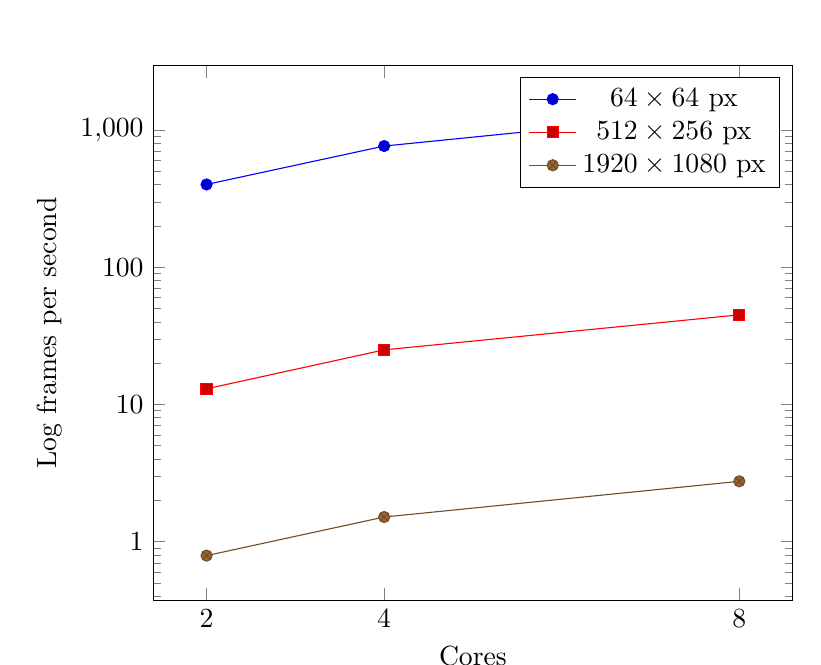
\begin{tikzpicture}
	 \begin{semilogyaxis}[
	 	 width=0.8\textwidth,
	     log ticks with fixed point,
	     xlabel=Cores,
	     ylabel=Log frames per second,
		     xtick = {2,4,8}
		 ]
		 \addplot plot coordinates {
		    (2, 402)
		    (4, 766)
		    (8, 1394)
		 };
		 \addplot plot coordinates {
		    (2, 13)
		    (4, 25 )
		    (8, 45)
		 };
		 \addplot plot coordinates {
		    (2, 0.79)
		    (4, 1.51)
		    (8, 2.75)
		 };
 
 
		 \legend{$64\times64$ px\\
		 $512\times256$ px\\
		 $1920\times1080$ px\\}

		 \end{semilogyaxis}
	\end{tikzpicture}
	\caption{Running the tunnel kernel.}	
	\label{fig:kernel_tunnel_fps}
\end{figure}


The figures \ref{fig:kernel_tunnel_fps}, and \ref{fig:kernel_green_screen_fps} display the relationship between frame rate, resolution and number of cores.
Both figures display that doubling the amount of core roughly doubles the frame rate.

For a configuration of cores, the time it takes to process one pixel is constant.
This means that the time to execute one kernel scales linearly with the resolution.
When the output resolution is increased, the amount of pixels to process increases quadratically.
As a consequence the frame rate decreases quadratically when the resolution grows.
  
For the target resolution for the project, which is $512\times256$, the project goal of maintaining 30 fps is achieved.

\section{Video output}
The Demolicious system can output to a screen using HDMI.
The minimum resolution permitted by the HDMI protocol is $640\times480$,
but the size of the data memory limits the actual resolution to $512\times256$ pixels.
The rest of the screen is padded with a checker pattern.
Most of the time the output image is correct.
However, the output image is distorted under certain conditions.
\begin{figure}[H]
	\centering
	\includegraphics[width=0.8\textwidth]{../results/diagrams/flicker.jpg}
	\caption{Flickering when running the tunnel kernel. This picture was exposed over two frames.}
	\label{fig:flickering}
\end{figure}
Some kernels exhibit intermittent flickering (Figure \ref{fig:flickering}).
The exact reason for why this occurs is unclear, but
it can be observed that the flicker contains parts of the last frame. 
This may be caused by a failure in the synchronization mechanism in the video unit.

Since the GPU has priority on memory access, the video unit may get starved for data.
When the video unit is starved the buffer containing pixels to output will underflow.
For the duration of the starve, a line containing the previous pixel on the bus will be displayed on the screen.

\section{Single vs double buffering}

Screen tearing is a visual artifact where parts of two consecutive frames are displayed at the same time.
This occurs because the video unit reads the frame buffer before the GPU has finished rendering it.  
In figure \ref{fig:single_buffering} the artifact can be observed, occurrences are marked with red circles.

\begin{figure}[H]
	\centering
	\includegraphics[width=0.5\textwidth]{../results/diagrams/single_buffering.png}
	\caption{Single buffering.}
	\label{fig:single_buffering}
\end{figure}
Double buffering is a technique to remove this artifact.
As the name implies two independent frame buffers are used.
While one frame buffer is being read and displayed on screen, 
the next frame is rendered to an off-screen frame buffer.
Once the frame has finished rendering the frame buffers are swapped, and the frame is displayed by the video unit.
In figure \ref{fig:double_buffering} it can be observed that double buffering improves the quality of the image substantially.
The image in the figure does have some artifacts, but the ones caused by single buffering are no longer present.
\begin{figure}[H]
	\centering
	\includegraphics[width=0.5\textwidth]{../results/diagrams/double_buffering.png}
	\caption{Double buffering.}
	\label{fig:double_buffering}
\end{figure}

\section{Power efficiency}

With a power draw of \SI{0.353}{W} for a Demolicious setup of 8 cores \ref{table:scalability},
it is in the interest of nature to keep it spinning for as short as possible.
By quickly and efficiently executing the kernel at hand, the GPU can reduce its total static power consumption.
Reducing the dynamic consumption however, is more difficult.
The current GPU architecture will execute nops when no kernels are active, keping dynamic power consumption sligthly lower than average, as no memory requests need to be served.
Therefore, Demolicious has been designed with the goal \ref{tab:goals} of allowing the host system to sleep as much as possible.

The Giant Gecko micro controller used as the host device has four different energy modes, each lower energy mode more efficient, but more constrained.
Deeper power levels may conserve more power, but require a longer time to wake up.
EM0 is normal operation, while EM2 (Deep sleep mode) is the deepest power level with acceptable wake-up times for our usecase (less than 2 ms) \cite{efm-referencemanual}.

There are two different sleep patterns used by the MCU based on the executing program:
\begin{enumerate}
  \item
    A visual animation or similar, rendering at a known target FPS.
    The MCU can stay at energy mode EM2 when kernels are executing, waking at fixed intervals to update and relaunch kernels.
  \item
    Programs working on some large dataset, where it is beneficial to tightly pack kernel execution, reducing GPU idling.
    The host device can therefore enter EM2 after launching a kernel, using the kernel complete pin to trigger an interrupt, waking the host device from sleep.
\end{enumerate}


Now for some numbers!
Let's say we're targeting 30 FPS on the tunnel kernel.
The kernel itself takes 3 ms to complete, when rendered at 64 x 64 resolution.
Kernel launch overhead is negligible.
This allows the CPU to spend 90 \% of its time in EM1 or 2, netting an average of (NUMBER * 0.40 + OTHERNUMBER * 0.60) power consumption.

For the throughput-intensive kernel, say the kernel itself takes 20ms to complete.
\todo{How much time does the MCU spend executing?}
Kernel launch overhead is 5\si\micro s, resulting in a 95 \% idle time that can be spent sleeping.
This averages to a power consumption of NUMBER.


Finally, the system can run for SOME HOURS on external batteries, mainly being limited by the GPU power draw.

\todo{software related power considerations? Sleeping MCU while kernel sleeps, awsm silicon labs stuff? In addition, perhaps some elaborations on energy use inside the GPU? Identifying energy critical systems.}

\subsection{PCB stuff MOVE THIS}

The system is powered by a EH-70p USB charger for the Nikon Coolpix S2700 camera \cite[p. 196]{usb-charger}.
This charger outputs a 5 V voltage and delivers 550 mA.
This gives the power input an upper bound of power consumption at $550mA * 5V = 2.75W$.

Based on checking the memory datasheet \cite{SRAM-datasheet}, page 4, the average current drawn from the SRAM is 100mA.
At two components, the memory energy consumption becomes $2 * 100mA * 3.3V = 660mW$, which makes them the most energy demanding part of the computer. 


\end{document}


% DISCUSSION
\documentclass[../main/report.tex]{subfiles}
\begin{document}
\chapter{Discussion}

\subfile{../discussion/design_process.tex}

%\section{PCB}
%Split project schematics into several connected docs for the sake of modularity. Find some overarching hardware requirements and from there, related application notes and hardware considerations. Then some components and footprints that fit...ish with these docs.
%Finally place components and route the wires between them digitally and order the PCB and components

\section{Power Considerations}

The system is powered by a 5V mini usb connection that delivers 550mA \todo{picture of the cable spec? Or something similar. A listing of the cable's spec}
This gives a theoretic maximum power consumption of $550mA$ $*$ $5V$ $=$ $2.75W$

\todo{Add actual power consumption, either based on datasheets or physical measurements?}
\todo{software related power considerations? Sleeping MCU while kernel sleeps, awsm silicon labs stuff? In addition, perhaps some elaborations on energy use inside the GPU? Identifying energy critical systems.}

\section{"Jaktstart"}

Not everyone can start at the same time

\section{Redundancy design choices or w/e}
What did we end up needing?
What could we have used, that we didn't think of.

\section{Does the computer make sense?}
Is the design sane?
Were we idiots?
Have we seen the light?

\section{Can we even saturate the memory bus?}
Do you even SRAM?
Or is memory the big bottleneck

\section{SRAM bottleneck}
HDMI vs. the GPU?
Will the HDMI be fine with always being second in line?

\end{document}


% CONCLUSION
\documentclass[../main/report.tex]{subfiles}
\begin{document}
\chapter{Conclusion}

We designed and implemented a graphics processing unit inspired system,
capable of executing a large amount of threads fast enough to display graphics to a display over HDMI.

The final system meets all the requirements set in the beginning of the project.
The goal of at least 30 FPS has been reached for several kernels,
at the target screen resolution of 512x256 pixels when running with 8 processor cores.

There is still room for further improvement of the computer, which will be detailed in the next section.

This project has been extremely challenging and demanding,
and has given the group as a whole great insight into the inner workings of computers,
and GPUs specifically.

\end{document}


% WORK PROCESS
\input{work_process/work_process.tex}

\printbibliography

\newpage

\appendix
%APPENDIX A
\section{Appendix A}

Appendices go here


% Fan fiction
\chapter{Yaman Fan Fiction}
TBD.



\end{document}
